\begin{questions}
\question{
Heaviside step
}
\begin{solution}
  Let's analyze the given integral
  \begin{equation}
    \Theta(x) = \int_{-\infty}^x \delta(y)dy.
    \label{int:1}
  \end{equation}

  From the hint we know that
  \begin{equation}
    f(x_0) = \int_{-\infty}^\infty f(x)\delta(x-x_0)dx,
  \end{equation}
  moreover, we know that if $x_0 \in (a,b)$ then
  \begin{equation}
    f(x_0) = \int_{a}^b f(x)\delta(x-x_0)dx,
    \label{int:2}
  \end{equation}
  if we compare eqs. \ref{int:2} and \ref{int:1} we will see that $x_0 = 0$, and $f(x) := 1$. Finally, let's remember that $\delta(x-x_0)$ is zero for all $x$ except $x_0$. Now we are ready to solve this.
  if $0\notin(-\infty,x)$ then $\Theta(x) = 0$, because $\delta(y)=0, \quad \forall y\in(-\infty,x)$. If $0\in(-\infty,x)$ then using eq. \ref{int:2} we conclude that $\Theta(x) = f(x) = 1$. Hence
  \begin{equation}
    \Theta(x) =
    \begin{cases}
      0 & x<0, \\
      1 & x>0.
   \end{cases}
  \end{equation}
  We can see the plot in fig. \ref{heavi}

\begin{center}
  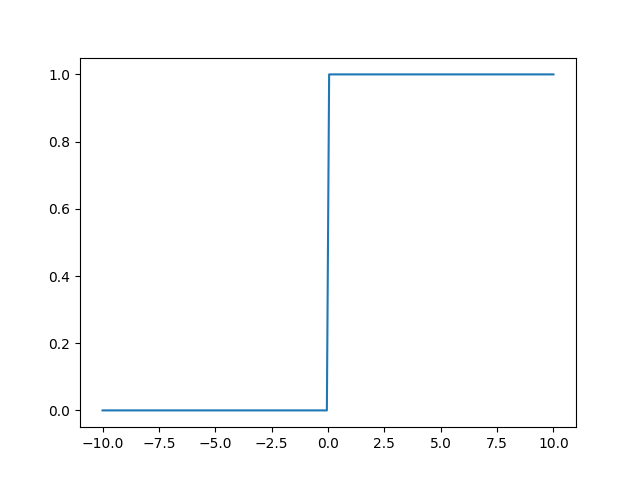
\includegraphics[width=75mm]{heavi}
\end{center}
   \captionof{figure}{Plot of the function defined in eq. \ref{int:1}.}\label{heavi}\vspace{0.5cm}
\end{solution}

\question{Fermi function}
\begin{solution}
  Consider the Fermi function
  \begin{equation}
    n(x) = \frac{1}{1+ e^{(x-\mu)/k_B T}}.
    \label{ferm}
  \end{equation}
  And let us analyze the behavior of $n(x)$. First consider the case $x<\mu$, then $x-\mu < 0$. If $T\rightarrow0$ then the factor $(x-\mu)/k_B T \rightarrow - \infty$, and $e^{(x-\mu)/k_B T} \rightarrow 0$ and as a consequence $1/(1+ e^{(x-\mu)/k_B T}) \rightarrow 1$ .

  On the other hand if $x-\mu > 0$ the factor $(x-\mu)/k_B T \rightarrow  \infty$ as $T\rightarrow0$, and therefore $e^{(x-\mu)/k_B T} \rightarrow \infty $ causing $1/(1+ e^{(x-\mu)/k_B T}) \rightarrow 0$

  So we see that in the limit $T\rightarrow0$
  \begin{equation}
    n(x) =
    \begin{cases}
      1 & x - \mu < 0, \\
      0 & x - \mu > 0.
   \end{cases}
  \end{equation}
  Now just multiplying the conditions by a $-1$ factor we will have
  \begin{equation}
    n(x) = \Theta (\mu - x)
    \begin{cases}
      0 & \mu - x < 0,\\
      1 & \mu - x > 0.  \quad_\blacksquare
   \end{cases}
  \end{equation}

  Now let's take the derivative of eq. \ref{ferm}.
  \begin{equation}
    \begin{aligned}[b]
      \frac{d}{dx} \left(1+ e^{(x-\mu)/k_B T}\right)^{-1} &= -(1+ e^{(x-\mu)/k_B T})^2e^{(x-\mu)/k_B T}\frac{1}{k_BT}, \\
      &= -\frac{e^{(x-\mu)/k_B T}}{k_BT (1+ e^{(x-\mu)/k_B T})^2}.
    \end{aligned}
  \end{equation}
  if $x-\mu < 0$ then
  \begin{eqnarray}
    \lim_{T\rightarrow 0} e^{(x-\mu)/k_B T} = 0,\\
    \lim_{T\rightarrow 0} \frac{1}{(1+ e^{(x-\mu)/k_B T})^2} = 1\\
    \lim_{T\rightarrow 0} \frac{e^{(x-\mu)/k_B T}}{k_BT } = 0,
  \end{eqnarray}
  and as a consequence
  \begin{eqnarray}
    \hlgreen{\lim_{T\rightarrow 0} \frac{dn(x)}{dx} = 0.}
  \end{eqnarray}
  If $x-\mu > 0$ then
  \begin{eqnarray}
    \lim_{T\rightarrow 0} e^{(x-\mu)/k_B T} = \infty,\\
    \lim_{T\rightarrow 0} \frac{1}{(1+ e^{(x-\mu)/k_B T})^2} \approx \lim_{T\rightarrow 0} \frac{1}{(e^{(x-\mu)/k_B T})^2} \\
    \lim_{T\rightarrow 0} -\frac{e^{(x-\mu)/k_B T}}{k_BT (1+ e^{(x-\mu)/k_B T})^2}. \approx \lim_{T\rightarrow 0} -\frac{1}{k_BTe^{(x-\mu)/k_B T}} = 0.
  \end{eqnarray}
  and as a consequence
  \begin{eqnarray}
    \hlgreen{\lim_{T\rightarrow 0} \frac{dn(x)}{dx} = 0.}
  \end{eqnarray}
  So, \textbf{for both cases the derivative tends to zero.}
\end{solution}
\end{questions}

% \includegraphics[width=75mm]{}
%
%
%  \captionof{figure}{}\label{}\vspace{0.5cm}
